\documentclass[10pt, titlepage]{article}
\usepackage[utf8]{inputenc}
\usepackage[T1]{fontenc}
\usepackage{amsmath}
\usepackage{amssymb}
\usepackage{calrsfs}
\usepackage{graphicx}
\graphicspath{ {figure/} }
\DeclareMathAlphabet{\pazocal}{OMS}{zplm}{m}{n}
\newcommand{\Hh}{\pazocal{H}}
\newcommand{\Gg}{\pazocal{G}}


%opening
\title{\textbf{Esercizio 1}}
\author{Danilo Bondì, Alfredo Guarnieri, Filippo Quarenghi}
%nodate
\date{}

\begin{document}

%\maketitle
\section*{To Do}
\begin{enumerate}
\item IMPLEMENTAZIONE: calcolo coefficiente trasmissione punto 1

\item plot coeff trasmissione metodo punto 1 vs pacchetti (qualche punto)
\end{enumerate}
\newpage


\section*{Testo dell'esercizio}
Si consideri la Hamiltoniana
$$ \Hh = -\frac{1}{2} \frac{ d^2}{dx^2} - V(x) $$
con potenziale assegnato da
$$
V(x)  = \begin{cases}
        0       & \mbox{se } x<-b \\
        4/b^2   & \mbox{se } -b \leq x \leq b \\
        0       & \mbox{se } x>b \\
         \end{cases}
$$
Sia $V0 = 4/b^2$. Siano:
$$
\begin{cases}
    \mbox{ZonaI} & = \{x<-b \} \\
    \mbox{ZonaII} & = \{-b \leq x \leq b\} \\
    \mbox{ZonaIII} & = \{x>b\}
\end{cases} $$

\bigskip
\begin{enumerate}
  \item Diagonalizzare un'opportuna versione discreta di H con eig. Quindi cercare di
  estrarre il coefficiente di trasmissione dagli autovalore/vettori in funzione dell'energia
  o del numero d'onda, confrontando con il risultato analitico esatto.

  \item Ripetere la procedura con un potenziale smooth come la barriera gaussiana e confrontare
  con il coefficiente di trasmissione calcolato come in classe (con il metodo
  dei pacchetti d'onda).
\end{enumerate}

Come mai questo metodo non funziona con $V(x)$?


\section*{Primo punto}
\subsection*{Introduzione teorica}

Si vuole studiare il problema agli autovalori:
$$ \Hh\psi = E \psi $$
%
Siano $k^2 = 2E$ e  $q^2 = 2(E-V0)$. La soluzione analitica più generale è data da:
%
$$
\psi_k(x) =
    \begin{cases}
        Ae^{ikx}+Be^{-ikx} & \mbox{in ZonaI} \\
        \phi(x) & \mbox{in ZonaII} \\
        Ce^{ikx}+De^{-ikx} & \mbox{in ZonaIII} \\
    \end{cases}
$$
%
\bigskip
Non siamo per il momento interessati alla ZonaII, quindi indichiamo con
$\phi(x)$ la $\psi_k(x)$ in tale zona, che a rigore sarebbe
    $$\phi(x)= Ee^{iqx}+Fe^{-iqx}$$
Le costanti $A,B,C,D$ sono determinate dalle condizioni di raccordo di continuità della
funzione d'onda e della sua derivata nei punti $x=\pm b$.\\
Si osserverà che dalla diagonalizzazione della versione discreta della Hamiltoniana
(vedi sezione apposita) risultano autofunzioni a parità definita (pari o dispari).
Allora, senza perdita di generalità, si pone la ulteriore condizione di simmetria alle $\psi_k$, che porta:
$$\begin{cases}
    A = D, \qquad  B = C = (\tau + \rho)A &\mbox{per funzioni pari} \\
    A = -D, \quad B = -C = -(\tau + \rho)A &\mbox{per funzioni dispari}\\
\end{cases}$$
Per la conservazione del flusso di probabilità, si possono riscrivere nella seguente forma:
$$
    \begin{pmatrix} C \\ B \end{pmatrix} =
    \begin{pmatrix} \tau & \rho \\ \rho & \tau \end{pmatrix} \cdot
    \begin{pmatrix} A \\ D \end{pmatrix} = \quad (S)\cdot \begin{pmatrix} A \\ D \end{pmatrix}
$$
Ove la matrice S è una matrice unitaria, che di conseguenza verifica le condizioni:
$$ \tau\rho^* + \tau^*\rho = 0 \quad,\quad |\tau|^2 + |\rho|^2 = 1$$
(Si è indicato con $z^*$ il numero complesso coniugato di $z$). Segue immediatamente che:
$$ |\tau \pm \rho|^2 = |\tau|^2 + |\rho|^2 + \tau\rho^* + \tau^*\rho = |\tau|^2 + |\rho|^2 + 0 = 1$$
Cioè $\tau \pm \rho$ differiscono per una fase:
$$ |\tau \pm \rho|^2 = 1 \Rightarrow (\tau \pm \rho) = e^{2i\theta^\pm}$$
Si osservi che poichè $A,B,C,D$ dipendono dagli autostati $\psi_k$, anche le fasi $\theta^\pm$ dipenderanno dall'autovalore $k$.\\
Si vuole quindi cercare una stima numerica di $\theta\pm$ per determinare $\tau$ da:
    $$ (\tau \pm \rho) = e^{2i\theta^\pm} \Rightarrow \tau = 1/2(e^{2i\theta^+}+e^{-2i\theta^-})$$
    $$ \Rightarrow \tau^2 = \sin^2(\theta^+ - \theta^-)$$
(due conti per dimostrarlo plis) (OCCHIO che esce un coseno)
\\
Il coefficiente di trasmissione sarà qundi dato da:
    $$T = \tau^2$$

\subsection*{Stima delle Fasi}
Si vuole stimare numericamente le fasi $\theta^\pm$, a partire dagli autovettori
calcolati dalla $\Hh$ discretizzata. Gli autovettori sono combinazioni pari e dispari
di onde piane con la stessa frequenza, quindi corrispondono rispettivamente a coseni e seni.
    $$ \psi_k^{odd} = \begin{cases}
        A\sin(kx + \theta^-_k) & \mbox{in ZonaI} \\
        A\sin(kx + \theta^+_k) & \mbox{in ZonaIII} \\
    \end{cases}
    \quad
    \psi_k^{even} = \begin{cases}
        A\cos(kx + \theta^-_k) & \mbox{in ZonaI} \\
        A\cos(kx + \theta^+_k) & \mbox{in ZonaIII} \\
    \end{cases}
    $$

\begin{paragraph}{Primo Metodo}
Si vuole fittare i dati con seni e coseni di opportuna frequenza $k$
e fase da determinare (parametro di fit). Si definiscono allora:\\
  In ZonaI = $\{x<-b\}$, sia
        $$f^{even}_k(y) = \int_{-\infty}^{-b} | A\cos(kx+y)-\psi_k^{even}(x)| \mathrm d x $$
        $$f^{odd}_k(y) = \int_{-\infty}^{-b} | A\sin(kx+y)-\psi_k^{odd}(x)| \mathrm d x $$
  In ZonaIII = $\{x<-b\}$, sia
        $$g^{even}_k(y) = \int_{b}^{+\infty} |A\cos(kx+y)-\psi_k^{even}(x)| \mathrm d x $$
        $$g^{odd}_k(y) = \int_{b}^{+\infty} |A\sin(kx+y)-\psi_k^{odd}(x)| \mathrm d x $$
Si ha immediatamente che:
    $$ \theta^-_k = y \mbox{ t.c. } f_k(\theta^-_k) = 0 $$
    $$ \theta^+_k = y \mbox{ t.c. } g_k(\theta^+_k) = 0 $$
\end{paragraph}
Si troverà che:
    $$ \theta^+_k = -\theta^-_k = \theta_k $$
Quindi:
$$ \psi_k^{odd} = \begin{cases}
    A\sin(kx - \theta_k) & \mbox{in ZonaI} \\
    A\sin(kx + \theta_k) & \mbox{in ZonaIII} \\
\end{cases}
\quad
\psi_k^{even} = \begin{cases}
    A\cos(kx - \theta_k) & \mbox{in ZonaI} \\
    A\cos(kx + \theta_k) & \mbox{in ZonaIII} \\
\end{cases}
$$

\begin{paragraph}{Secondo Metodo}
Si considerino i punti $x = \pm 2\pi$, siano $y(\pm 2\pi)$ i valori degli autovettori
numerici in quei punti, separatamente pari e dispari. Si ha allora che:
$$ \begin{cases}
    y^{odd}(2\pi)   = \sin(k2\pi  + \theta_o^+)  & \Rightarrow \theta_o^+ = \arcsin(y^{odd}(2\pi)) - k2\pi\\
    y^{odd}(-2\pi)  = \sin(-k2\pi + \theta_o^-)  & \Rightarrow \theta_o^- = \arcsin(y^{odd}(-2\pi)) + k2\pi\\
    y^{even}(2\pi)  = \cos(k2\pi  + \theta_e^+)  & \Rightarrow \theta_e^+ = \arccos(y^{even}(2\pi)) - k2\pi\\
    y^{even}(-2\pi) = \cos(-k2\pi + \theta_e^-)  & \Rightarrow \theta_e^- = \arccos(y^{even}(-2\pi)) + k2\pi\\
\end{cases}$$
\end{paragraph}
Di seguito il plot del risultato\\
%% Sarebbe bello che stesse sulla stessa pagina
\begin{figure}[h]
  \centering
  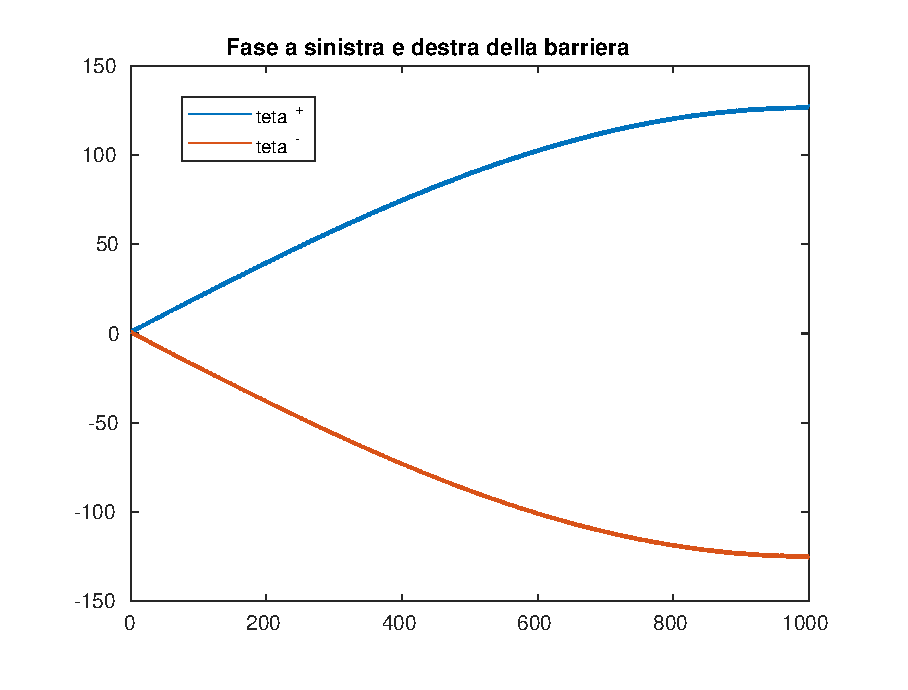
\includegraphics{fasi.eps}
\end{figure}
%
\newpage
\subsection*{Risultati}
Di seguito il plot del coefficiente di trasmissione calcolato numericamente contro
il risultato analitico

%% Immagine da mettere sotto la frase, possibilmente in una unica pagina
\begin{figure}[h]
  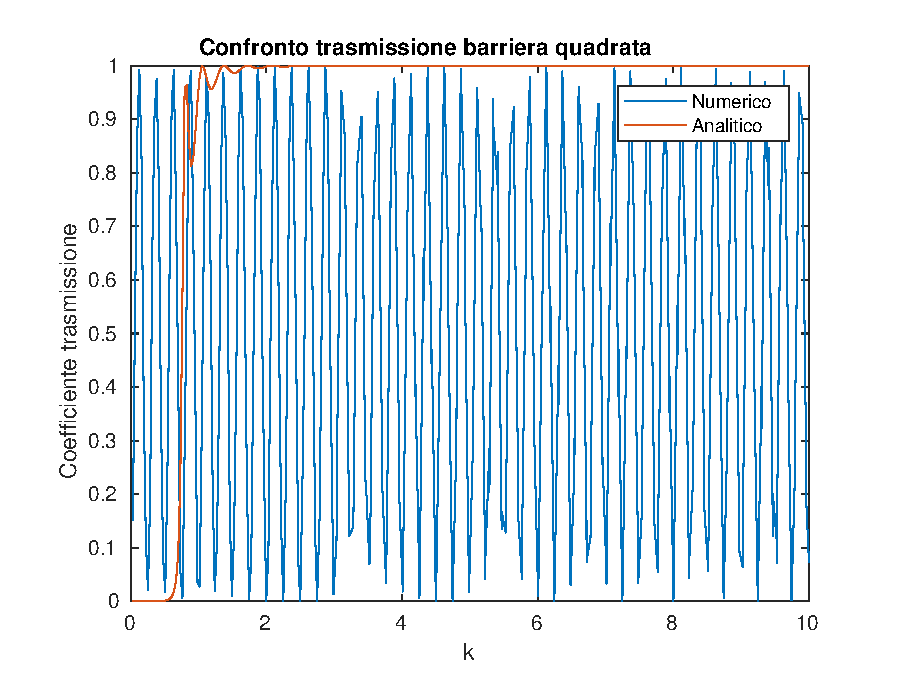
\includegraphics{tr_coeff_square.eps}
\end{figure}

\input{AppChapter1}
\section*{Secondo punto}
\subsection*{Metodo dei pacchetti d'onda}
Il metodo consiste nel far evolvere temporalmente un dato iniziale a pacchetto
d'onda nel potenziale stabilito e nel calcolare, dopo un opportuno tempo $t_0$,
la porzione di funzione d'onda che è oltre la barriera. Il tempo $t_0$ deve essere tale
da permettere il passaggio del pacchetto oltre la barriera, ma evitare riflessioni
ai bordi della scatola $[-L,L]$.
In tal caso, supponendo un pacchetto incidente da sinistra a destra,
il coefficiente di trasmissione sarà semplicemente
    $$ T = \frac{\int_b^L |\psi(x,t_0)|^2\mathrm d x}{\int_{-L}^L |\psi(x,t_0)|^2\mathrm d x} $$
Si vuole confrontare questo metodo con il metodo trovato al punto precedente,
per una barriera di potenziale di tipo gaussiano.\\
Essendo un pacchetto d'onda una sovrapposizione lineare di più onde stazionarie,
non possiede un momento ben definito. Il confronto verrà allora fatto tra il valor medio
del momento di un dato pacchetto, contro il corrispettivo autovalore
del metodo precedente (o quello che più gli si avvicina).
Si possono riscontrare le seguenti difficoltà:
\begin{itemize}
    \item pacchetti poco localizzati presentano problemi nella rilessione contro la barriera
    e nell'autointerferenza con i bordi della scatola
    \item pacchetti troppo localizzati presentano valori del momento
    molto dispersi a causa del principio di indeterminazione:
    questo introduce errori di approssimazione maggiori nel valutarne il valor medio
\end{itemize}
\bigskip
Di seguito i risultati.\\
\subsection*{Confronto dei due metodi}

\subsection*{Conclusioni}
Il metodo dei pacchetti d'onda non funziona con il potenziale a barriera quadrata
del punto 1, a causa della discontinuità del potenziale. La discontinuità
impedisce una buona riflessione del pacchetto d'onda incidente, risultando nella
permanenza di parte dell'onda nella zona della barriera per un lungo tempo.
Questo altera il calcolo dell'integrale della definizione di $T$ perchè
viene omessa una parte importante dell'onda. Il tempo che l'onda residua nella barriera
impiega a spegnersi è molto maggiore del tempo che il resto del pacchetto impiega
ad arrivare ai bordi della scatola e riflettersi, interagendo con sè stesso.
Il metodo risulta quindi inefficiente. Di seguito alcuni plot che mostrano
quanto detto.

% Metterle in un unico 'box' tutte e tre affiancate
\begin{figure}[h]
 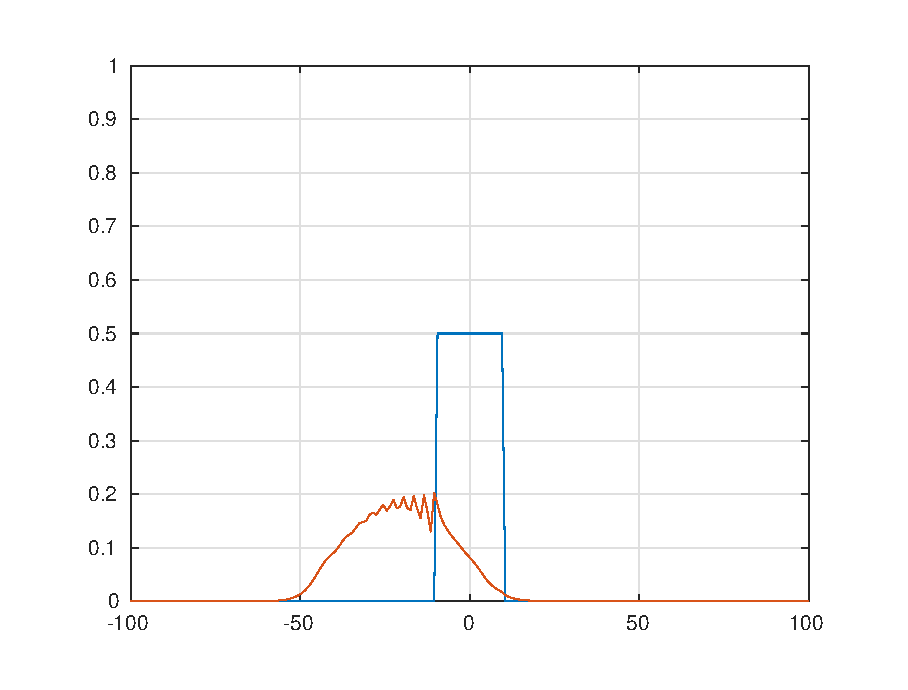
\includegraphics{square_transmission1.eps}
\end{figure}
\begin{figure}[h]
 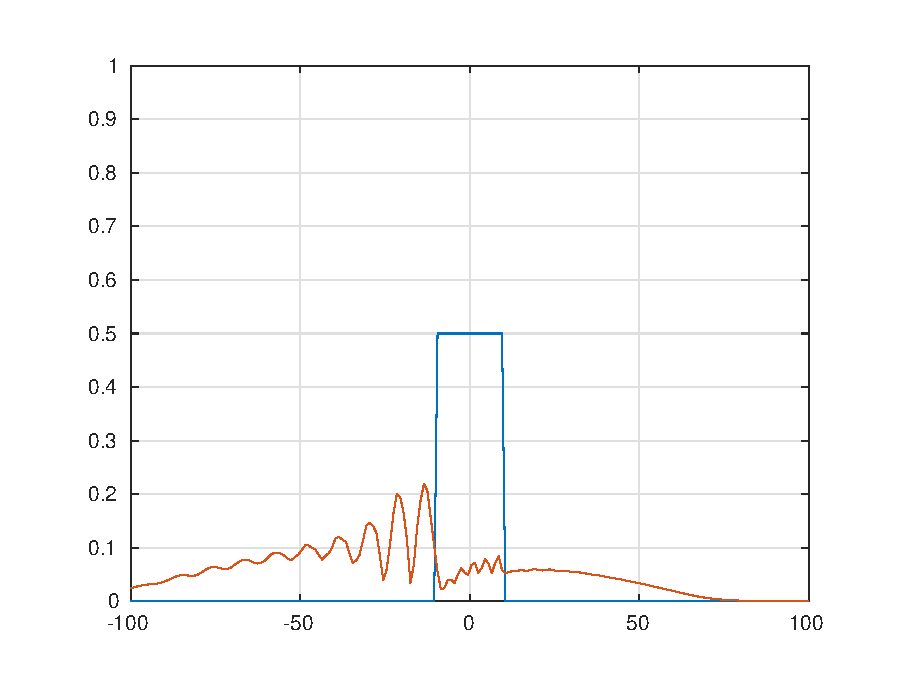
\includegraphics{square_transmission2.eps}
\end{figure}
\begin{figure}[h]
 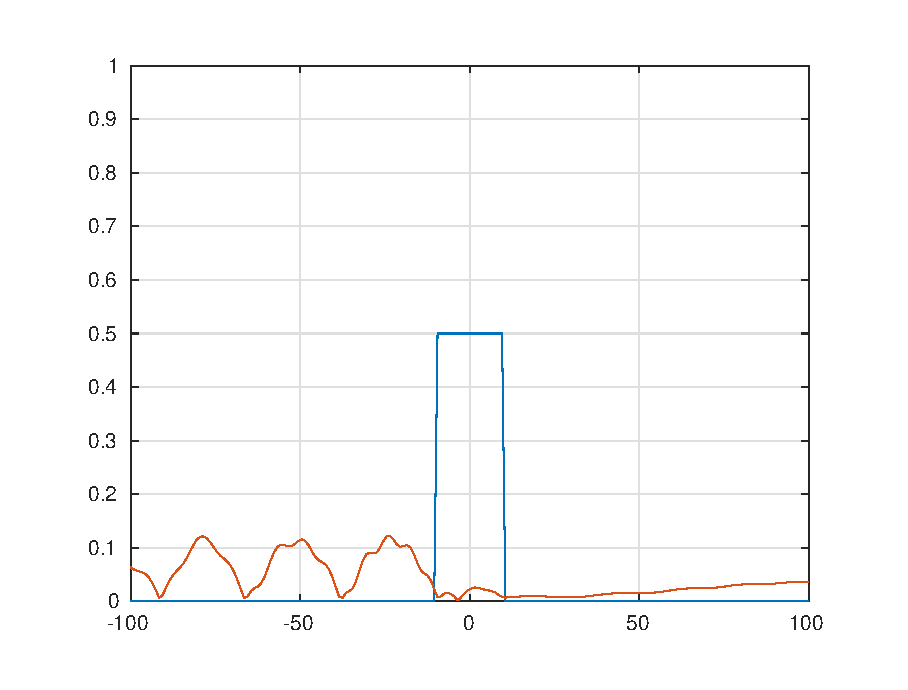
\includegraphics{square_transmission3.eps}
\end{figure}


\end{document}
